\documentclass[twocolumns]{IEEEtran}
\usepackage{tikz}
\tikzstyle{box}=[rectangle,draw=black, ultra thick, minimum size=1cm]
\usepackage{algorithm}
\usepackage{algorithmic}

\author{Erdal Sidal Dogan, Alp Gokcek \\ MEF University \\ \today}
\title{Max-Subarray Sum Problem and Solution Algorithms}


\begin{document}
	\maketitle
	\begin{abstract}
		Maximum Subarray Sum is a well-known problem in the field of computer science. There are multiple number of solution algorithms with different complexities. In this paper, we demonstrated and compared 3 of these algorithms with quadratic, linear, and logarithmic complexities.
	\end{abstract}
\section{The Problem}
The Maximum Subarray Sum problem is the task of finding the contiguous subarray with largest sum in a given array of integers. Each number in the array could be positive, negative, or zero. For example: Given the array $[-2, 1, -3, 4, -1, 2, 1, -5, 4]$ the solution would be $[4, -1, 2, 1]$ with a sum of 6.
\section{Solutions}
\subsection{Brute-Force Approach}
This is the most intuitive solution to anyone. You basically traverse over the array and compare every possible combination of start and end index for the soultion array.\\ \\


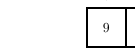
\begin{tikzpicture}[transform canvas={scale=.5}, trim left=-1cm]
[%%%%%%%%%%%%%%%%%%%%%%%%%%%%%%
box/.style={rectangle,draw=black, ultra thick, minimum size=0.5cm},
]%%%%%%%%%%%%%%%%%%%%%%%%%%%%%%

\foreach \x/\y in {0/9, 1/5,2/13,3/19,4/12,5/8,6/7,7/4,8/21,9/2,10/6,11/11}
\node[box] at (\x,0){\y};

\draw[->,very thick] (0,1.2) --  node[above,yshift=2mm]{start} (0,.7);
\draw[->,very thick] (1,1.2) --  node[above,yshift=2mm]{end} (1,.7);
\end{tikzpicture} 
\\ \\ \\
The \textit{start} index will be incremented by 1 everytime the \textit{end} index reaches the end of the array. Then the \textit{end} index will start from the element right next to the start element. At every iteration the sum between \textit{start} and \textit{end} indexes will be calculated. Hence, the maximum sum will be determined by computing every sum for the every possible sub-array. The complexity of this algorithm is $\mathcal{O}(n^3)$. With a little improvement we can convert this algorithm to be $\mathcal{O}(n^2)$. Instead of calculating the sum between two array indicies at every iteration from scratch, we know that the current sum will be the (current element + previous sum). Consequently, eliminating the loop which is used for calculating the sum from the algorithm will reduce the time complexity.
\newpage
\begin{algorithm}
	\caption{Brute-Force}
	\begin{algorithmic} 
		\STATE $y \leftarrow 1$ 
		\IF{$n < 0$}
		\STATE $X \leftarrow 1 / x$
		\STATE $N \leftarrow -n$
		\ELSE
		\STATE $X \leftarrow x$
		\STATE $N \leftarrow n$
		\ENDIF
		\WHILE{$N \neq 0$}
		\IF{$N$ is even}
		\STATE $X \leftarrow X \times X$
		\STATE $N \leftarrow N / 2$
		\ELSE[$N$ is odd]
		\STATE $y \leftarrow y \times X$
		\STATE $N \leftarrow N - 1$
		\ENDIF
		\ENDWHILE
	\end{algorithmic}
\end{algorithm}



\end{document}